\documentclass[13pt,ignorenonframetext,aspectratio = 1610]{beamer}
\setbeamertemplate{caption}[numbered]
\setbeamertemplate{caption label separator}{: }
\setbeamercolor{caption name}{fg=normal text.fg}
\beamertemplatenavigationsymbolsempty
\usepackage{lmodern}
\usepackage{amssymb,amsmath}
% packages
\usepackage{amsfonts, algorithm, algpseudocode, dsfont,
	pgfplots, tikz, tikzscale, ulem, xcolor}
\usetikzlibrary{arrows,shapes,positioning,external}
\pgfplotsset{compat=1.15}

\usepackage{ifxetex,ifluatex}
\usepackage{fixltx2e} % provides \textsubscript
\ifnum 0\ifxetex 1\fi\ifluatex 1\fi=0 % if pdftex
  \usepackage[T1]{fontenc}
  \usepackage[utf8]{inputenc}
\else % if luatex or xelatex
  \ifxetex
    \usepackage{mathspec}
  \else
    \usepackage{fontspec}
  \fi
  \defaultfontfeatures{Ligatures=TeX,Scale=MatchLowercase}
    \setmainfont[]{Roboto Light}
    \setmonofont[Mapping=tex-ansi]{Roboto Mono}
\fi
\usefonttheme{serif} % use mainfont rather than sansfont for slide text
% use upquote if available, for straight quotes in verbatim environments
\IfFileExists{upquote.sty}{\usepackage{upquote}}{}
% use microtype if available
\IfFileExists{microtype.sty}{%
\usepackage{microtype}
\UseMicrotypeSet[protrusion]{basicmath} % disable protrusion for tt fonts
}{}
\newif\ifbibliography
\hypersetup{
            pdftitle={Sampling Probability Distributions},
            pdfauthor={Jon Fintzi},
            pdfborder={0 0 0},
            breaklinks=true}
%\urlstyle{same}  % Use monospace font for urls
\usepackage{graphicx,grffile}
\makeatletter
\def\maxwidth{\ifdim\Gin@nat@width>\linewidth\linewidth\else\Gin@nat@width\fi}
\def\maxheight{\ifdim\Gin@nat@height>\textheight0.8\textheight\else\Gin@nat@height\fi}
\makeatother
% Scale images if necessary, so that they will not overflow the page
% margins by default, and it is still possible to overwrite the defaults
% using explicit options in \includegraphics[width, height, ...]{}
\setkeys{Gin}{width=\maxwidth,height=\maxheight,keepaspectratio}

% Prevent slide breaks in the middle of a paragraph:
\widowpenalties 1 10000
\raggedbottom

\AtBeginPart{
  \let\insertpartnumber\relax
  \let\partname\relax
  \frame{\partpage}
}
\AtBeginSection{
  \ifbibliography
  \else
    \let\insertsectionnumber\relax
    \let\sectionname\relax
    \frame{\sectionpage}
  \fi
}
\AtBeginSubsection{
  \let\insertsubsectionnumber\relax
  \let\subsectionname\relax
  \frame{\subsectionpage}
}

\setlength{\parindent}{0pt}
\setlength{\parskip}{6pt plus 2pt minus 1pt}
\setlength{\emergencystretch}{3em}  % prevent overfull lines
\providecommand{\tightlist}{%
  \setlength{\itemsep}{0pt}\setlength{\parskip}{0pt}}
\setcounter{secnumdepth}{0}


\title[Sampling Probability Distributions]{Sampling Probability Distributions}
\subtitle{From conjugacy to Hamiltonian Monte Carlo}
\author[
Jon Fintzi
]{Jon Fintzi}
\institute[
Biostatistics Research Branch
]{
Biostatistics Research Branch \\
National Institute of Allergy and Infectious Diseases\\
National Institutes of Health
}
\date[
08/19/19
]{
August 19, 2019
}

% ------------------------------------------------------------------------------------------------
% BELOW ARE MY ADDITIONS
% ------------------------------------------------------------------------------------------------

% ------------------------------------------------------------------------------------------------
% CUSTOM COMMANDS
% ------------------------------------------------------------------------------------------------
\newcommand{\Var}{\mathrm{Var}}
\newcommand{\E}{\mathrm{E}}
\newcommand{\mr}[1]{\mathrm{#1}}
\newcommand{\mb}[1]{\mathbf{#1}}
\newcommand{\mi}[1]{\mathit{#1}}
\newcommand{\bs}[1]{\boldsymbol{#1}}
\newcommand{\rmd}{\mr{d}}
\newcommand{\ind}[1]{\mathds{1}_{\left \lbrace#1\right \rbrace}}
\newcommand{\deriv}[2]{\frac{\rmd#1}{\rmd#2}}
\newcommand{\pdiv}[2]{\frac{\partial#1}{\partial#2}}
\newcommand{\diag}{\mr{diag}}
\newcommand{\wtil}[1]{\widetilde{#1}}
\newcommand{\what}[1]{\widehat{#1}}

% ------------------------------------------------------------------------------------------------
%	PACKAGE LIST
% ------------------------------------------------------------------------------------------------
\usepackage{
booktabs,
%fontspec,
graphicx,
multicol,
pgfplots,
ragged2e,
tabularx,
wasysym,
hyperref,
hanging,
multirow,
eso-pic,
}

\usepackage[export]{adjustbox}
% ------------------------------------------------------------------------------------------------
%	GRAPHICS PATH
% ------------------------------------------------------------------------------------------------
\graphicspath{{./figs/}}


% ------------------------------------------------------------------------------------------------
%	TABLE OF CONTENTS
% ------------------------------------------------------------------------------------------------
\useoutertheme[subsection=false,shadow]{miniframes}
\setbeamertemplate{section in toc}[sections numbered]
\setbeamertemplate{subsection in toc}[subsections numbered]

% ------------------------------------------------------------------------------------------------
%	ITEMIZE
% ------------------------------------------------------------------------------------------------
\setbeamertemplate{itemize item}{$\bullet$}
\setbeamertemplate{itemize subitem}{$\circ$}
\setbeamertemplate{itemize subsubitem}{$\bullet$}

\setlength{\parskip}{0.5em}

% ------------------------------------------------------------------------------------------------
%	COLORS
% ------------------------------------------------------------------------------------------------

% sthlm Colors
\definecolor{sthlmLightBlue}{RGB}{0,91,150}
\definecolor{sthlmBlue}{RGB}{3,57,108}
\definecolor{sthlmDarkBlue}{RGB}{1,31,75}
\definecolor{sthlmLightRed}{RGB}{143,39,39}
\definecolor{sthlmRed}{RGB}{124,0,0}
\definecolor{sthlmLightYellow}{RGB}{255,204,0}
\definecolor{sthlmYellow}{RGB}{255,149,0}
\definecolor{sthlmPurple}{RGB}{64,0,64}
\definecolor{sthlmGreen}{RGB}{25,77,51}
\definecolor{sthlmGrey}{RGB}{142,142,147}
\definecolor{sthlmLightGrey}{RGB}{233,233,233}
\definecolor{sthlmDarkGrey}{RGB}{61,61,70}

% General
\setbeamercolor{normal text}{fg=sthlmDarkGrey}
\hypersetup{colorlinks=true, urlcolor=sthlmDarkBlue, linkcolor=sthlmDarkGrey, citecolor=sthlmDarkBlue}
\setbeamercolor{structure}{fg=sthlmDarkGrey}
\setbeamercolor{alerted text}{fg=sthlmRed}
\setbeamercolor{example text}{fg=white}
\setbeamercolor{copyright text}{fg=sthlmLightBlue}
\setbeamercolor{palette primary}{fg=sthlmDarkGrey}
\setbeamercolor{palette secondary}{fg=sthlmDarkGrey,bg=sthlmLightGrey}
\setbeamercolor{palette tertiary}{fg=black,bg=sthlmDarkGrey}
\setbeamercolor{palette quaternary}{fg=white, bg=sthlmDarkGrey}

\setbeamercolor{mini frame}{bg=sthlmLightGrey}
\setbeamercolor{section in head/foot}{fg=sthlmDarkGrey, bg=sthlmLightGrey}

% Titlepage
\setbeamercolor{title}{parent=normal text}
\setbeamercolor{subtitle}{parent=normal text}
\setbeamercolor{institute}{parent=normal text}

% Content
\setbeamercolor{frametitle}{parent=palette quaternary}

% Blocks
\setbeamercolor{block title}{fg=white,bg=sthlmBlue}
\setbeamercolor{block body}{fg=sthlmDarkGrey, bg=sthlmLightGrey}
\setbeamercolor{block title example}{fg=white, bg=sthlmGreen}
\setbeamercolor{block body example}{fg=sthlmDarkGrey, bg=sthlmLightGrey}
\setbeamercolor{block title alerted}{fg=white, bg=sthlmLightRed}
\setbeamercolor{block body alerted}{fg=sthlmDarkGrey, bg=sthlmLightGrey}

% Notes
\setbeamercolor{note page}{fg=sthlmDarkGrey,bg=sthlmLightGrey}
\setbeamercolor{note title}{fg=white, bg=sthlmDarkGrey}
\setbeamercolor{note date}{parent=note title}

% Page Number
\setbeamercolor{page number in head/foot}{fg=sthlmDarkGrey}

\setbeamercolor{qed}{fg=sthlmGrey}
\setbeamercolor{itemize item}{fg=sthlmDarkBlue}
\setbeamercolor{itemize subitem}{fg=sthlmDarkBlue}
\setbeamercolor{itemize subsubitem}{fg=sthlmDarkBlue}

% ------------------------------------------------------------------------------------------------
%	FONTS
% ------------------------------------------------------------------------------------------------

% General

%% Declare fontfamilys
%\if@doNoFlama%
%	% Sans serif math option
%	\if@doSans%
%	% Sans serif math
%		\usepackage{fontspec}%
%		\setmainfont{Arial Regular}%
%	\else%
%		% Serif math
%		\usefonttheme{professionalfonts}%
%		\usepackage[no-math]{fontspec}%
%	\fi%
%	
%	\newfontfamily\Light{Arial Regular}%
%	\newfontfamily\Book{Arial Black Regular}%
%	\newfontfamily\bfseries{Arial Bold}%
%	\setsansfont{Arial Regular}%
%\else%
%	% Sans serif math option
%	\if@doSans%
%	% Sans serif math
%		\usepackage{fontspec}%
%		\setmainfont{FlamaLight}%
%	\else%
%		% Serif math
%		\usefonttheme{professionalfonts}%
%		\usepackage[no-math]{fontspec}%
%	\fi%
%	
%	\newfontfamily\Light{FlamaLight}%
%	\newfontfamily\Book{FlamaBook}%
%	\newfontfamily\bfseries{FlamaMedium}%
%	\setsansfont{FlamaLight}%
%	%\newfontfamily\texttt{SourceCodePro-Light}
%\fi%
%
%%\renewcommand\UrlFont{\texttt}
%
%% Font sizes
%
%% Titlepage
%\setbeamerfont{title}{family=\bfseries,size=\fontsize{24}{26}}
%\setbeamerfont{subtitle}{family=\Light,size=\fontsize{14}{18}}
%\setbeamerfont{subtitle}{size=\fontsize{14}{18}}
%\setbeamerfont{date}{size=\fontsize{9}{11}}
%\setbeamerfont{author}{family=\bfseries,size=\fontsize{13}{15}}
%\setbeamerfont{institute}{size=\fontsize{09}{10}}
%
%% Section
%\setbeamerfont{section title}{size*={39pt}{24pt}, family = \bfseries, series=\bfseries}% Content
%\setbeamerfont{frametitle}{family=\bfseries,size=\large}
%\setbeamerfont{copyright text}{family=\Light,size=\tiny}
%\setbeamerfont{block title}{family=\Book,size=\large}
%\setbeamerfont{block title alerted}{family=\Book,size=\large}
%\setbeamerfont{alerted text}{family=\bfseries}
%
%%Captions
%\setbeamerfont{caption name}{family=\Book}




%% ------------------------------------------------------------------------------------------------
%%	FONT ASSIGMENTS
%% ------------------------------------------------------------------------------------------------
%% Title Page
%\newfontfamily\Light{Roboto Light}
%\setbeamerfont{title}{size=\LARGE, series=\bfseries}
%\setbeamerfont{subtitle}{family=\Light, size=\small, shape=\normalfont}
%\setbeamerfont{date}{family=\Light, size=\footnotesize}
%\setbeamerfont{author}{size=\small, series=\bfseries}
%\setbeamerfont{institute}{family=\Light, size=\scriptsize}
%
%% Section
%\setbeamerfont{section title}{size=\Huge}
%
%% Content
%\setbeamerfont{frametitle}{size=\Large, series=\bfseries}
%\setbeamerfont{copyright text}{size=\tiny}
%\setbeamerfont{block title}{size=\large, series=\bfseries}
%\setbeamerfont{block title alerted}{size=\large, series=\bfseries}
%\setbeamerfont{block title example}{size=\large, series=\bfseries}
%
%\setbeamerfont{caption}{size=\small}
%\setbeamerfont{caption name}{family=\small}

% ------------------------------------------------------------------------------------------------
%	FONT ASSIGMENTS
% ------------------------------------------------------------------------------------------------
% Title Page
%\newfontfamily\Light{Roboto Light}
\setbeamerfont{title}{size=\LARGE, series=\bfseries}
\setbeamerfont{subtitle}{size=\normalsize, shape=\normalfont}
\setbeamerfont{date}{size=\normalsize}
\setbeamerfont{author}{size=\normalsize, series=\bfseries}
\setbeamerfont{institute}{size=\small}

% Section
\setbeamerfont{section title}{size=\Huge}

% Content
\setbeamerfont{frametitle}{size=\Large, series=\bfseries}
\setbeamerfont{copyright text}{size=\tiny}
\setbeamerfont{block title}{size=\large, series=\bfseries}
\setbeamerfont{block title alerted}{size=\large, series=\bfseries}
\setbeamerfont{block title example}{size=\large, series=\bfseries}

\setbeamerfont{caption}{size=\small}
\setbeamerfont{caption name}{family=\small}

% ------------------------------------------------------------------------------------------------
%	TITLE PAGE
% ------------------------------------------------------------------------------------------------

\newcommand\AtPageUpperRight[1]{\AtPageUpperLeft{%
 \put(\LenToUnit{\paperwidth},\LenToUnit{0\paperheight}){#1}%
 }}%
\newcommand\AtPageLowerRight[1]{\AtPageLowerLeft{%
 \put(\LenToUnit{\paperwidth},\LenToUnit{0\paperheight}){#1}%
 }}%

%\AddToShipoutPictureBG*{% Add picture to current page
%  \AtStockLowerLeft{% Add picture to lower-left corner of paper stock
%    \includegraphics[width=\stockwidth,height=\stockheight]{tiger}}% http://latex.tug.org/texlive/devsrc/Master/texmf-dist/doc/generic/pstricks/images/tiger.eps
%}

% Titlepage structure
\def\maketitle{\ifbeamer@inframe\titlepage\else\frame[plain]{\titlepage}\fi}
\def\titlepage{\usebeamertemplate{title page}}
\setbeamertemplate{title page}
%\frame[plain]{\titlepage}
{
	% Add background to title page
  	%\AddToShipoutPictureFG*{\includegraphics[width=\paperwidth]{backgroundiegs.pdf}}
	%\AddToShipoutPictureFG*{
	%	\AtPageLowerRight{\put(-95, 0){
	%		\includegraphics[width=.2\paperwidth]{title_graphic.pdf}}}}
	%\AddToShipoutPictureFG*{\includegraphics[width=\paperwidth]{youngmetro_logo.png}}
	\begin{minipage}[b][\paperheight]{\textwidth}
	%\vspace*{5mm}
	%\includegraphics[height=14mm]{./logo}\par
	\vspace*{20mm}
	\ifx\insertsubtitle\@empty%
	\else%
		{\usebeamerfont{title}\usebeamercolor[fg]{title}\MakeUppercase{\inserttitle}\parskip0pt\par}%
	\fi%
	\ifx\insertsubtitle\@empty%
	\else%
		{\usebeamerfont{subtitle}\usebeamercolor[fg]{subtitle}\insertsubtitle\par}%
		\vspace*{5mm}
	\fi%
	\ifx\insertdate\@empty%
	\else%
		{\usebeamerfont{date}\usebeamercolor[fg]{date}\insertdate\par}%
	\fi% 
	
	\vfill
	
	\ifx\insertauthor\@empty%
	\else%
		{\usebeamerfont{author}\usebeamercolor[fg]{author}\insertauthor\par}%
	\fi%
	\ifx\insertinstitut\@empty%
	\else%
		\vspace*{1mm}
		{\usebeamerfont{institute}\usebeamercolor[sthlmDarkGrey]{institute}\insertinstitute\par}%
	\fi% 
	\vspace*{5mm}
	\end{minipage}
}

% ------------------------------------------------------------------------------------------------
%	SECTION PAGES
% ------------------------------------------------------------------------------------------------

% Make Sectionhead uppercase
\newcommand{\insertsectionHEAD}{%
	\expandafter\insertsectionHEADaux\insertsectionhead}
	\newcommand{\insertsectionHEADaux}[3]{\MakeUppercase{#3}
}

\if@doSectionPage\@empty
\else
% Insert frame with section title at every section start
\AtBeginSection[]
{
\begingroup
\setbeamercolor{background canvas}{bg=sthlmDarkGrey}
\begin{frame}[plain]
\centering
\vfill\usebeamerfont{section title}\textcolor{white}{\insertsectionHEAD}\vfill
\end{frame}
\endgroup
}
\fi

% ------------------------------------------------------------------------------------------------
%	HEADLINE
% ------------------------------------------------------------------------------------------------
\makeatletter
\def\progressbar@progressbar{} % the progress bar
\newcount\progressbar@tmpcounta% auxiliary counter
\newcount\progressbar@tmpcountb% auxiliary counter
\newdimen\progressbar@pbht %progressbar height
\newdimen\progressbar@pbwd %progressbar width
\newdimen\progressbar@tmpdim % auxiliary dimension

\progressbar@pbwd=\paperwidth
\progressbar@pbht=1.25ex

% the progress bar
\def\progressbar@progressbar{%
    \progressbar@tmpcounta=\insertframenumber
    \progressbar@tmpcountb=\inserttotalframenumber
    \progressbar@tmpdim=\progressbar@pbwd
%    \divide\progressbar@tmpdim by 100
%    \multiply\progressbar@tmpdim by \progressbar@tmpcounta
%    \divide\progressbar@tmpdim by \progressbar@tmpcountb
%    \multiply\progressbar@tmpdim by 100
  \begin{tikzpicture}[very thin]

    \shade[top color=sthlmLightGrey,bottom color=sthlmLightGrey,middle color=sthlmLightGrey]
      (0pt, 0pt) rectangle ++ (\progressbar@pbwd, \progressbar@pbht);

      \shade[draw=sthlmDarkBlue,top color=sthlmDarkBlue,bottom color=sthlmDarkBlue,middle color=sthlmDarkBlue] %
        (0pt, 0pt) rectangle ++ (\progressbar@tmpdim, \progressbar@pbht);

  \end{tikzpicture}%
}

\setbeamertemplate{headline}{

  \begin{beamercolorbox}[wd=\paperwidth,ht=1ex,center,dp=0ex]{sthlmLightGrey}%
    \progressbar@progressbar%
  \end{beamercolorbox}%
}

%% ------------------------------------------------------------------------------------------------
%%	FRAME TITLE IN ALL CAPS (MAC: USE "? + ? + }" to uncomment section
%% ------------------------------------------------------------------------------------------------
%\setbeamertemplate{frametitle}
%{
%\begin{beamercolorbox}[wd=\paperwidth,leftskip=0.3cm,rightskip=0.3cm,ht=3ex,dp=1.5ex]{frametitle}
%	 \usebeamerfont{frametitle}\MakeUppercase{\insertframetitle}%
%\end{beamercolorbox}
%}

% ------------------------------------------------------------------------------------------------
%	FRAME TITLE IN TITLE CASE (MAC: USE "? + ? + {" to comment-out section
% ------------------------------------------------------------------------------------------------
\setbeamertemplate{frametitle}
{
\begin{beamercolorbox}[sep=0ex,wd=\paperwidth,leftskip=0.25cm,rightskip=0.3cm,ht=2.75ex,dp=1.375ex]{frametitle}
	 \usebeamerfont*{frametitle}{\insertframetitle}%
\end{beamercolorbox}
}


%\setbeamertemplate{block alerted begin}
%{
%  \setbeamercolor{item}{parent=block body alerted}
%  \par\vskip\medskipamount%
%  \begin{beamercolorbox}[sep=.5ex,dp=0.6ex,leftskip=0.5ex,rightskip=0.5ex]{block title alerted}
%    \usebeamerfont*{block title alerted}\insertblocktitle%
%  \end{beamercolorbox}%
%  {\parskip0pt\par}%
%  {\nointerlineskip\vskip-0.5pt}%
%  \usebeamerfont{block body alerted}%
%  \begin{beamercolorbox}[sep=.5ex,dp=0.6ex,leftskip=0.5ex,rightskip=0.5ex,vmode]{block body alerted}%
%}
%\setbeamertemplate{block alerted end}
%{\end{beamercolorbox}\vskip\smallskipamount}

% ------------------------------------------------------------------------------------------------
%	FOOTLINE
% ------------------------------------------------------------------------------------------------
\usenavigationsymbolstemplate{}
\setbeamertemplate{footline}
{
  \leavevmode%
  \hbox{%
  \begin{beamercolorbox}[sep=0.25ex,wd=.333333\paperwidth,ht=3.25ex,dp=1.25ex,left]{author in head/foot}%
    \usebeamerfont{author in head/foot}\insertshortauthor\expandafter\beamer@ifempty\expandafter{\beamer@shortinstitute}{}{~~--- \insertshortinstitute}
  \end{beamercolorbox}%
  \begin{beamercolorbox}[sep=0.5ex,wd=.333333\paperwidth,ht=3.25ex,dp=1.25ex,center]{title in head/foot}%
    \usebeamerfont{title in head/foot}\insertshorttitle
  \end{beamercolorbox}%
  \begin{beamercolorbox}[sep=0.5ex,wd=.333333\paperwidth,ht=3.25ex,dp=1.25ex,right]{date in head/foot}%
    %\usebeamerfont{date in head/foot}\insertshortdate{}\hspace*{2em}
    Page \insertframenumber{} %/ \inserttotalframenumber\hspace*{2ex} 
  \end{beamercolorbox}}%
  \vskip0pt%
}

% ------------------------------------------------------------------------------------------------
%	CAPTIONS
% ------------------------------------------------------------------------------------------------
\setbeamertemplate{caption label separator}{: }

% ------------------------------------------------------------------------------------------------
%	BLOCKS
% ------------------------------------------------------------------------------------------------
\setbeamertemplate{block begin}
{
  \setbeamercolor{item}{parent=block body}
  \par\vskip\medskipamount%
  \begin{beamercolorbox}[sep=.5ex,dp=0.6ex,leftskip=0.5ex,rightskip=0.5ex]{block title}
    \usebeamerfont*{block title}\insertblocktitle%
  \end{beamercolorbox}%
  {\parskip0pt\par}%
  {\nointerlineskip\vskip-0.5pt}%
  \usebeamerfont{block body}%
  \begin{beamercolorbox}[sep=.5ex,dp=0.6ex,leftskip=0.5ex,rightskip=0.5ex,vmode]{block body}%
}
\setbeamertemplate{block end}  
{\end{beamercolorbox}\vskip\smallskipamount}

\setbeamertemplate{block alerted begin}
{
  \setbeamercolor{item}{parent=block body alerted}
  \par\vskip\medskipamount%
  \begin{beamercolorbox}[sep=.5ex,dp=0.6ex,leftskip=0.5ex,rightskip=0.5ex]{block title alerted}
    \usebeamerfont*{block title alerted}\insertblocktitle%
  \end{beamercolorbox}%
  {\parskip0pt\par}%
  {\nointerlineskip\vskip-0.5pt}%
  \usebeamerfont{block body alerted}%
  \begin{beamercolorbox}[sep=.5ex,dp=0.6ex,leftskip=0.5ex,rightskip=0.5ex,vmode]{block body alerted}%
}
\setbeamertemplate{block alerted end}
{\end{beamercolorbox}\vskip\smallskipamount}

\setbeamertemplate{block example begin}
{
  \par\vskip\medskipamount%
  \begin{beamercolorbox}[sep=.5ex,dp=0.6ex,leftskip=0.5ex,rightskip=0.5ex]{block title example}
    \usebeamerfont*{block title example}\insertblocktitle%
  \end{beamercolorbox}%
  {\parskip0pt\par}%
  {\nointerlineskip\vskip-0.5pt}%
  \usebeamerfont{block body example}%
  \begin{beamercolorbox}[sep=.5ex,dp=0.6ex,leftskip=0.5ex,rightskip=0.5ex,vmode]{block body example}%
}
\setbeamertemplate{block example end}
{\end{beamercolorbox}\vskip\smallskipamount}

% ------------------------------------------------------------------------------------------------
%	BLOCK HOVERING ABOVE THE SLIDE
% ------------------------------------------------------------------------------------------------

\newcommand<>{\hover}[1]{\uncover#2{%
	\begin{tikzpicture}[remember picture,overlay]%
	\draw[fill,opacity=0.4] (current page.south west)
	rectangle (current page.north east);
	\node at (current page.center) {#1};
	\end{tikzpicture}}
	}

% ------------------------------------------------------------------------------------------------
%	VERTICALLY ALIGNED COLUMNS
% ------------------------------------------------------------------------------------------------
	
\usepackage{environ}% Required for \NewEnviron, i.e. to read the whole body of the environment

\newcounter{acolumn}%  Number of current column
\newlength{\acolumnmaxheight}%   Maximum column height


% `column` replacement to measure height
\newenvironment{@acolumn}[1]{%
    \stepcounter{acolumn}%
    \begin{lrbox}{\@tempboxa}%
    \begin{minipage}{#1}%
}{%
    \end{minipage}
    \end{lrbox}
    \@tempdimc=\dimexpr\ht\@tempboxa+\dp\@tempboxa\relax
    % Save height of this column:
    \expandafter\xdef\csname acolumn@height@\roman{acolumn}\endcsname{\the\@tempdimc}%
    % Save maximum height
    \ifdim\@tempdimc>\acolumnmaxheight
        \global\acolumnmaxheight=\@tempdimc
    \fi
}

% `column` wrapper which sets the height beforehand
\newenvironment{@@acolumn}[1]{%
    \stepcounter{acolumn}%
    % The \autoheight macro contains a \vspace macro with the maximum height minus the natural column height
    \edef\autoheight{\noexpand\vspace*{\dimexpr\acolumnmaxheight-\csname acolumn@height@\roman{acolumn}\endcsname\relax}}%
    % Call original `column`:
    \orig@column{#1}%
}{%
    \endorig@column
}

% Save orignal `column` environment away
\let\orig@column\column
\let\endorig@column\endcolumn

% `columns` variant with automatic height adjustment
\NewEnviron{acolumns}[1][]{%
    % Init vars:
    \setcounter{acolumn}{0}%
    \setlength{\acolumnmaxheight}{0pt}%
    \def\autoheight{\vspace*{0pt}}%
    % Set `column` environment to special measuring environment
    \let\column\@acolumn
    \let\endcolumn\end@acolumn
    \BODY% measure heights
    % Reset counter for second processing round
    \setcounter{acolumn}{0}%
    % Set `column` environment to wrapper
    \let\column\@@acolumn
    \let\endcolumn\end@@acolumn
    % Finally process columns now for real
    \begin{columns}[#1]%
        \BODY
    \end{columns}%
}

% ------------------------------------------------------------------------------------------------
%	IMAGES
% ------------------------------------------------------------------------------------------------

\newbox\mytempbox
\newdimen\mytempdimen

\newcommand\includegraphicscopyright[3][]{%
  \leavevmode\vbox{\vskip3pt\raggedright\setbox\mytempbox=\hbox{\includegraphics[#1]{#2}}%
    \mytempdimen=\wd\mytempbox\box\mytempbox\par\vskip1pt%
    \usebeamerfont{copyright text}{\usebeamercolor[fg]{copyright text}{\vbox{\hsize=\mytempdimen#3}}}\vskip3pt%
}}

\begin{document}

% Hide progress bar and footline on titlepage
\begin{frame}[plain]
\titlepage
\end{frame}

\begin{frame}{Happy Monday-Funday!}
\protect\hypertarget{happy-monday-funday}{}

\textbf{Last time:} \vspace{-0.1in}

\begin{itemize}
\tightlist
\item
  Bayesian inference \emph{always} starts with a model for the
  \textbf{joint distribution} of \(\theta\) and \(y\):.\vspace{-0.1in}
  \[\pi(\theta, y) = f(y|\theta)\pi(\theta) = \pi(\theta|y)m(y).\vspace{-0.1in}\]

  \begin{itemize}
  \tightlist
  \item
    \(\pi(\theta|y)\) is the \textbf{posterior distribution} of
    \(\theta\) given \(y\),
  \item
    \(f(y|\theta)\) is the \textbf{sampling distribution} for \(y\)
    given \(\theta\),
  \item
    \(\pi(\theta)\) is the \textbf{prior distribution} of \(\theta\),
  \item
    \(m(y)\) is the \textbf{marginal distribution} of \(y\).
  \end{itemize}
\item
  \textbf{Bayes rule} yields the \textbf{posterior distribution}
  \vspace{-0.1in}
  \[\pi(\theta|y) =  \frac{f(y,\theta)}{m(y)} = \frac{f(y|\theta)\pi(\theta)}{m(y)} \propto Likelihood\times Prior.\vspace{-0.1in}\].
\item
  All of the information used in the \emph{update} to our prior is
  encoded in the \textbf{likelihood},\vspace{-0.1in}
  \[L(\mb{y}|\theta) = \prod_{i=1}^N f(y_i|\theta).\vspace{-0.1in}\]

  \begin{itemize}
  \tightlist
  \item
    \emph{Likelihood principle}: implies proportional likelihoods encode
    equivalent updates for a single observer.
  \item
    Two people can have different epistemic uncertainty (different
    priors).
  \item
    The likelihood principle does not imply equivalent Bayesian
    inferences (corollary to Gelman, 2017).
  \end{itemize}
\end{itemize}

\end{frame}

\begin{frame}{Lecture 10 of Statistical Rethinking}
\protect\hypertarget{lecture-10-of-statistical-rethinking}{}

Key takeaways:\vspace{-0.1in}

\begin{itemize}
\tightlist
\item
  Bayes is all about the posterior distribution, not how you compute it.
\item
  Sometimes, we can't get the posterior analytically, but we can
  approximate it by sampling.
\item
  Samples also give us a way to approximate the distributions of
  complicated functionals of the posterior.
\item
  Markov Chain Monte Carlo is one way to sample.

  \begin{itemize}
  \tightlist
  \item
    Metropolis/Metropolis-Hastings.
  \item
    Hamiltonian Monte Carlo.
  \end{itemize}
\end{itemize}

\end{frame}

\begin{frame}{This Week}
\protect\hypertarget{this-week}{}

\textbf{Iterations on Bayesian analysis of binomial data}\vspace{-0.1in}

\begin{itemize}
\tightlist
\item
  Motivating example --- PREVAIL II Trial.
\item
  Analysis with conjugate priors, beta-binomial model.
\item
  Prior selection.
\item
  Analysis with non-conjugate priors.
\item
  First look at Stan if there's time.
\end{itemize}

\end{frame}

\begin{frame}{Motivating Example --- PREVAIL II Trial}
\protect\hypertarget{motivating-example-prevail-ii-trial}{}

\textbf{Context:}\vspace{-0.1in}

\begin{itemize}
\tightlist
\item
  2014--2016 Ebola virus disease (EVD) outbreak in Guinea, Liberia, and
  Sierra Leone.
\item
  Over 28,000 suspected or confirmed cases and 11,000 fatalities.
\item
  Urgent need to identify effective theraputics to reduce mortality.
\end{itemize}

\textbf{Partnership for Research on Ebola Virus in Liberia (PREVAIL) II
trial:}\vspace{-0.1in}

\begin{itemize}
\tightlist
\item
  Adaptive trial to determine the effectiveness of Zmapp, and possibly
  other agents, in reducing Ebola mortality.
\item
  Primary endpoint: 28 day mortality on optimized standard of care
  (oSOC) vs.~Zmapp + oSOC.
\item
  72 patients enrolled at sites in Liberia, Sierra Leone, Guinea, and
  the US. \vspace{-0.1in}

  \begin{itemize}
  \tightlist
  \item
    Overall mortality: 21/71 died (30\%),
  \item
    SOC alone: 13/35 (37\%),
  \item
    Zmapp + SOC: 8/36 (22\%).
  \end{itemize}
\item
  \sout{Super-duper} Barely Bayesian design (Proschan, 2016).
\end{itemize}

\end{frame}

\begin{frame}{Motivating Example --- PREVAIL II Trial}
\protect\hypertarget{motivating-example-prevail-ii-trial-1}{}

\textbf{Target of inference:} \(\pi(p_T,p_C|y_T,y_C)\), the posterior
distributions for probability of death on treatment (T) and control (C).
\vspace{-0.1in}

\begin{itemize}
\tightlist
\item
  \(p_T,p_C\): probabilities of 28 day mortality on T and C.
\item
  \(y_T,y_C\): \# of deaths on T and C.
\item
  \(N_T,N_C\): \# participants randomized to T and C.
\end{itemize}

\textbf{Some questions of interest:}\vspace{-0.1in}

\begin{itemize}
\tightlist
\item
  Evidence for Zmapp + oSOC more effective than oSOC alone:
  \(\Pr(p_T<p_C | y_T,y_C)\).
\item
  Effectiveness of Zmapp + oSOC, effectiveness of oSOC alone:
  \(\pi(p_T|y_T),\ \pi(p_C|y_C)\).
\end{itemize}

\end{frame}

\begin{frame}{A Simple Model for Count Data}
\protect\hypertarget{a-simple-model-for-count-data}{}

\textbf{Binomial count model:}\vspace{-0.1in}

\begin{itemize}
\tightlist
\item
  Arises as a model for \emph{independent} binary random variables
  (RVs), \(Z_i\in\lbrace 0,1\rbrace,\ i=1,\dots,N\), with \emph{common
  success probability}, \(p\).
\item
  Let \(Y = \sum_{i=1}^N Z_i\). The probability of seeing \(Y=y\)
  successes in \(N\) trials is \begin{align}
  \label{eqn:binom_pmf}
  \Pr(Y=y|p) &= \left(\begin{array}{c}N \\ y\end{array}\right)p^y(1-p)^{N-y}.\\
  &\propto p^y(1-p)^{N-y} \nonumber
  \end{align}
\item
  For fixed \(y\), we can view (\ref{eqn:binom_pmf}) as a function of
  \(p\) --- this is the \textbf{likelihood function}.
\item
  The maximum likelihood estimate (MLE), \(\what{p} = y/N\), is the
  value of \(p\) under which the observed data are most likely (i.e.,
  \(\what{p}\) maximizes the likelihood).
\end{itemize}

\end{frame}

\begin{frame}{A Simple Model for Count Data}
\protect\hypertarget{a-simple-model-for-count-data-1}{}

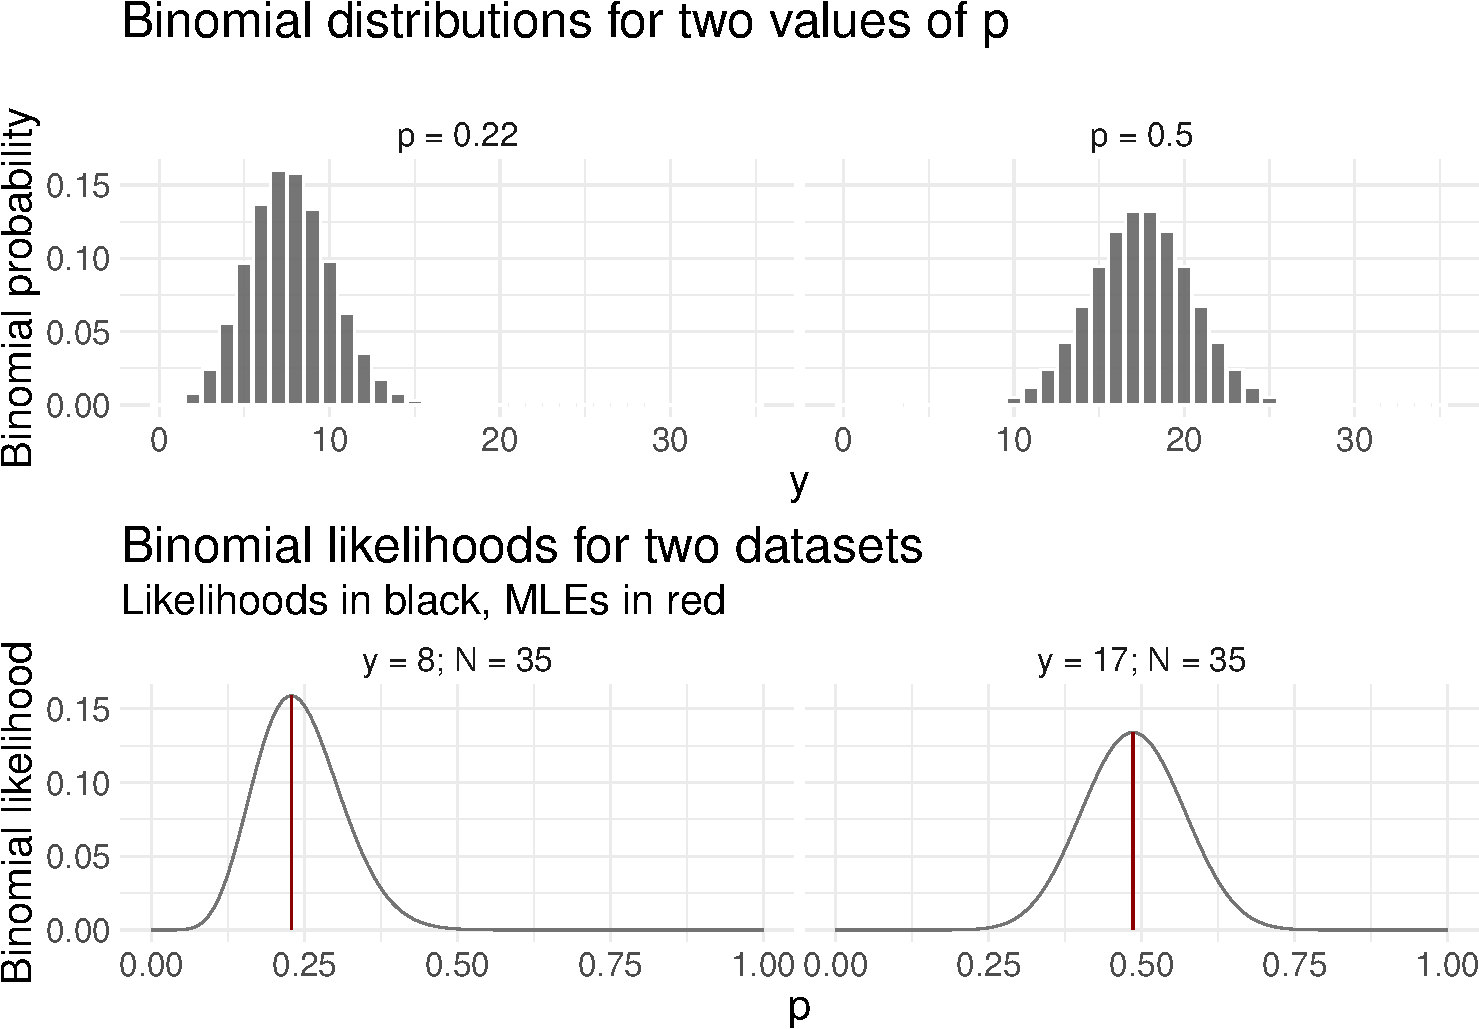
\includegraphics{sampling_probability_distributions_files/figure-beamer/binom_dists-1.pdf}

\end{frame}

\begin{frame}{Beta Distribution as a Prior for a Binomial Probability}
\protect\hypertarget{beta-distribution-as-a-prior-for-a-binomial-probability}{}

\textbf{Beta distribution}\vspace{-0.1in}

\begin{itemize}
\tightlist
\item
  If we though all values of \(p\) were equally likely, could take
  \(p\sim\mr{Unif}(0,1)\). In general, this is too restrictive.
\item
  More flexible: \(\theta\sim\mr{Beta}(a,b),\ \mr{with}\  a>0,b>0\),
  where\vspace{-0.1in} \begin{align}
  \pi(\theta|a,b) &= \frac{\Gamma(a+b)}{\Gamma(a)\Gamma{b}}p^{(a-1)}(1-p)^{b-1},\\
  &\propto p^{(a-1)}(1-p)^{b-1}, \nonumber
  \end{align} for \(0<p<1\) and where \(\Gamma(\cdot)\) is the gamma
  function\footnote<.->{\(\Gamma(z) = \int_0^\infty t^{z-1}e^{-t}\rmd t\),
    more on the Beta distribution
    \href{https://en.wikipedia.org/wiki/Beta_distribution}{here}.}.
\item
  \(p\sim\mr{Unif}(0,1)\) is equivalent to \(p\sim\mr{Beta}(1,1)\).
\item
  Moments: \vspace{-0.1in} \begin{align*}
   \E(p|a,b) &= \frac{a}{a+b},\\
   \Var(p|a,b) &= \frac{ab}{(a+b)^2(a+b+1)}.
  \end{align*}
\end{itemize}

\end{frame}

\begin{frame}{Beta Distribution as a Prior for a Binomial Probability}
\protect\hypertarget{beta-distribution-as-a-prior-for-a-binomial-probability-1}{}

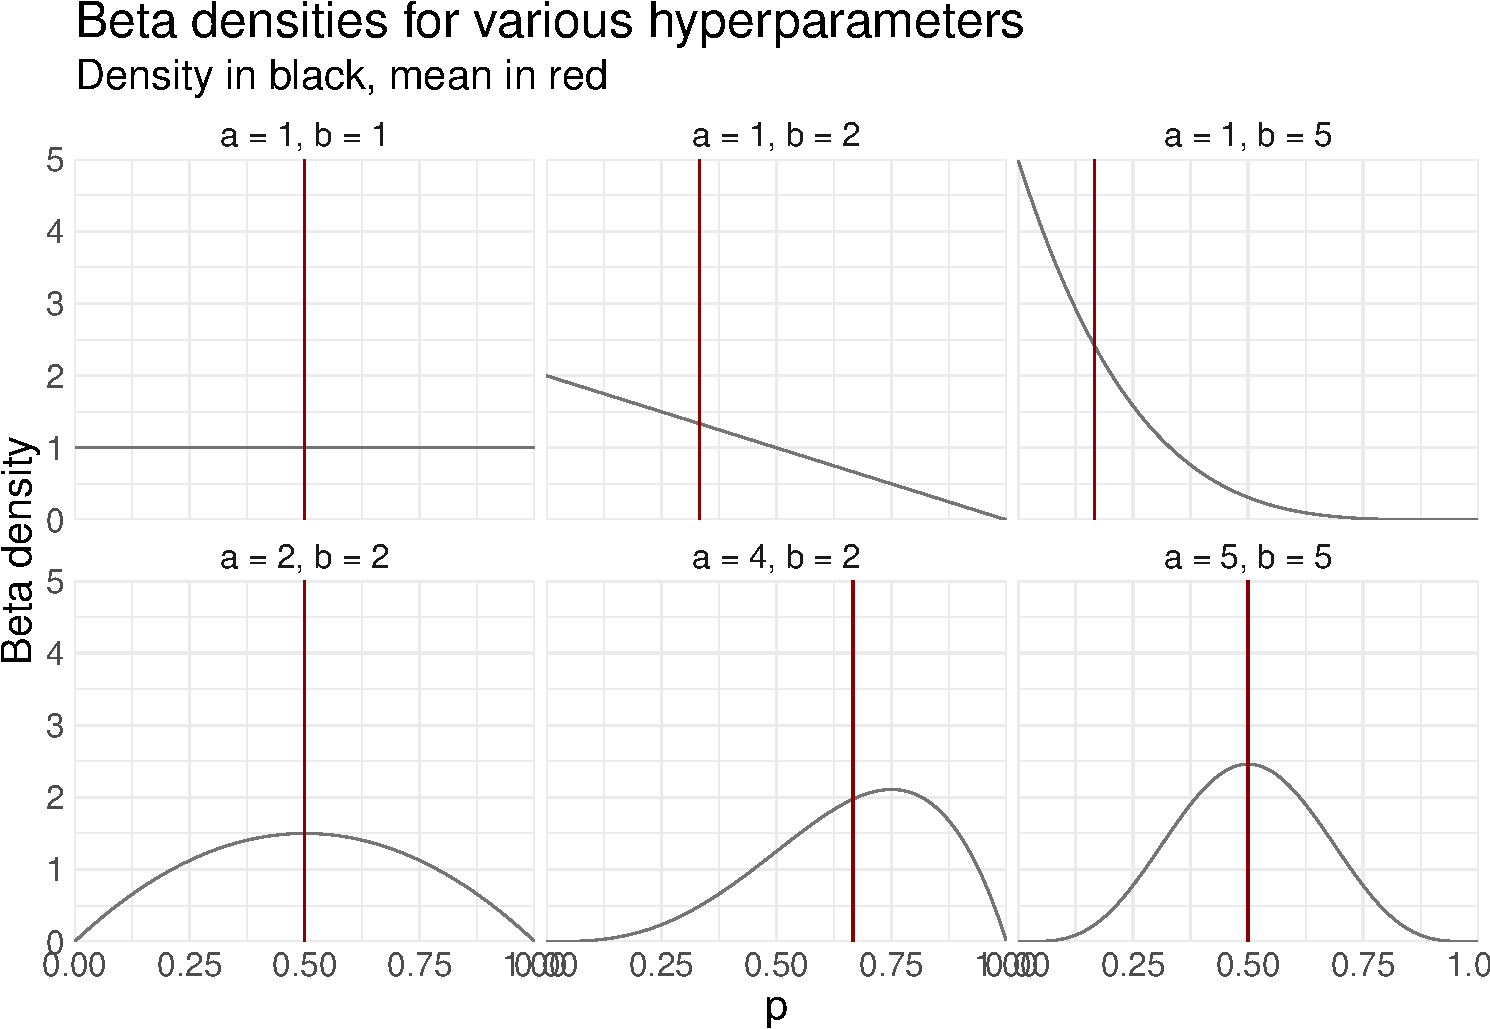
\includegraphics{sampling_probability_distributions_files/figure-beamer/beta_dists-1.pdf}

\end{frame}

\begin{frame}{Posterior Derivation}
\protect\hypertarget{posterior-derivation}{}

In the Beta-Binomial hierarchy, concentrate only on terms that involve
\(\theta\). \begin{align*}
\textcolor{green}{\pi(p|y)} &\propto \textcolor{blue}{L(y|p)}\textcolor{red}{\pi(p)}, \\ 
 &= \textcolor{blue}{p^y(1-p)^{N-y}} \times \textcolor{red}{p^{a-1}(1-p)^{b-1}},\\
 &= \textcolor{green}{p^{y+a-1}(1-p)^{N-y+b-1}},\\
 &= \textcolor{green}{p^{\wtil{a}-1}(1-p)^{\wtil{b}-1}},
\end{align*} where \(\wtil{a} = y+a\) and \(\wtil{b} = N-y+b\).

\begin{itemize}
\tightlist
\item
  The posterior takes the form of a \(\mr{Beta}(\wtil{a},\wtil{b})\)!
\item
  We say the prior is
  \href{https://en.wikipedia.org/wiki/Conjugate_prior}{\emph{conjugate}}
  when the posterior is of the same form as the prior.
\item
  Fun fact: all exponential family distributions have conjugate priors!
\end{itemize}

\end{frame}

\begin{frame}{PREVAIL II Posterior Distributions}
\protect\hypertarget{prevail-ii-posterior-distributions}{}

\begin{itemize}
\tightlist
\item
  Priors: \(p_T \sim \mr{Beta}(1,1)\) and \(p_C\sim\mr{Beta}(1,1)\).
\item
  Data: \(y_T = 8\) and \(y_C=13\), with \(N_T = 36\) and \(N_C=35\).
\item
  Posteriors: \(p_T|y_T\sim\mr{Beta}(9,29)\) and
  \(p_C|y_C\sim\mr{Beta}(14, 23).\)

  \begin{itemize}
  \tightlist
  \item
    Posterior medians (95\% Credible Intervals):

    \begin{itemize}
    \tightlist
    \item
      Zmapp + oSOC, \(p_T|y_T\) 0.23 (0.12, 0.38),
    \item
      oSOC alone, \(p_C|y_C\): 0.38 (0.23, 0.54).
    \item
      Risk difference, \(p_T-p_C\ |\ y_T,y_C\): -0.14 (-0.34, 0.06).
    \item
      Risk ratio, \(p_T/p_C\ |\ y_T,y_C\): 0.62 (0.29, 1.24).
    \item
      Odds ratio,
      \(\left[(p_T/(1-p_T))\ /\ (p_C/(1-p_C))\right]\ |\ y_T,y_C:\)
      \(0.50 (0.18, 1.36)\)
    \item
      \(\Pr(p_T<p_C|y_T,y_C)\approx 0.91\).
    \end{itemize}
  \end{itemize}
\end{itemize}

\end{frame}

\begin{frame}{PREVAIL II Posterior Distributions}
\protect\hypertarget{prevail-ii-posterior-distributions-1}{}

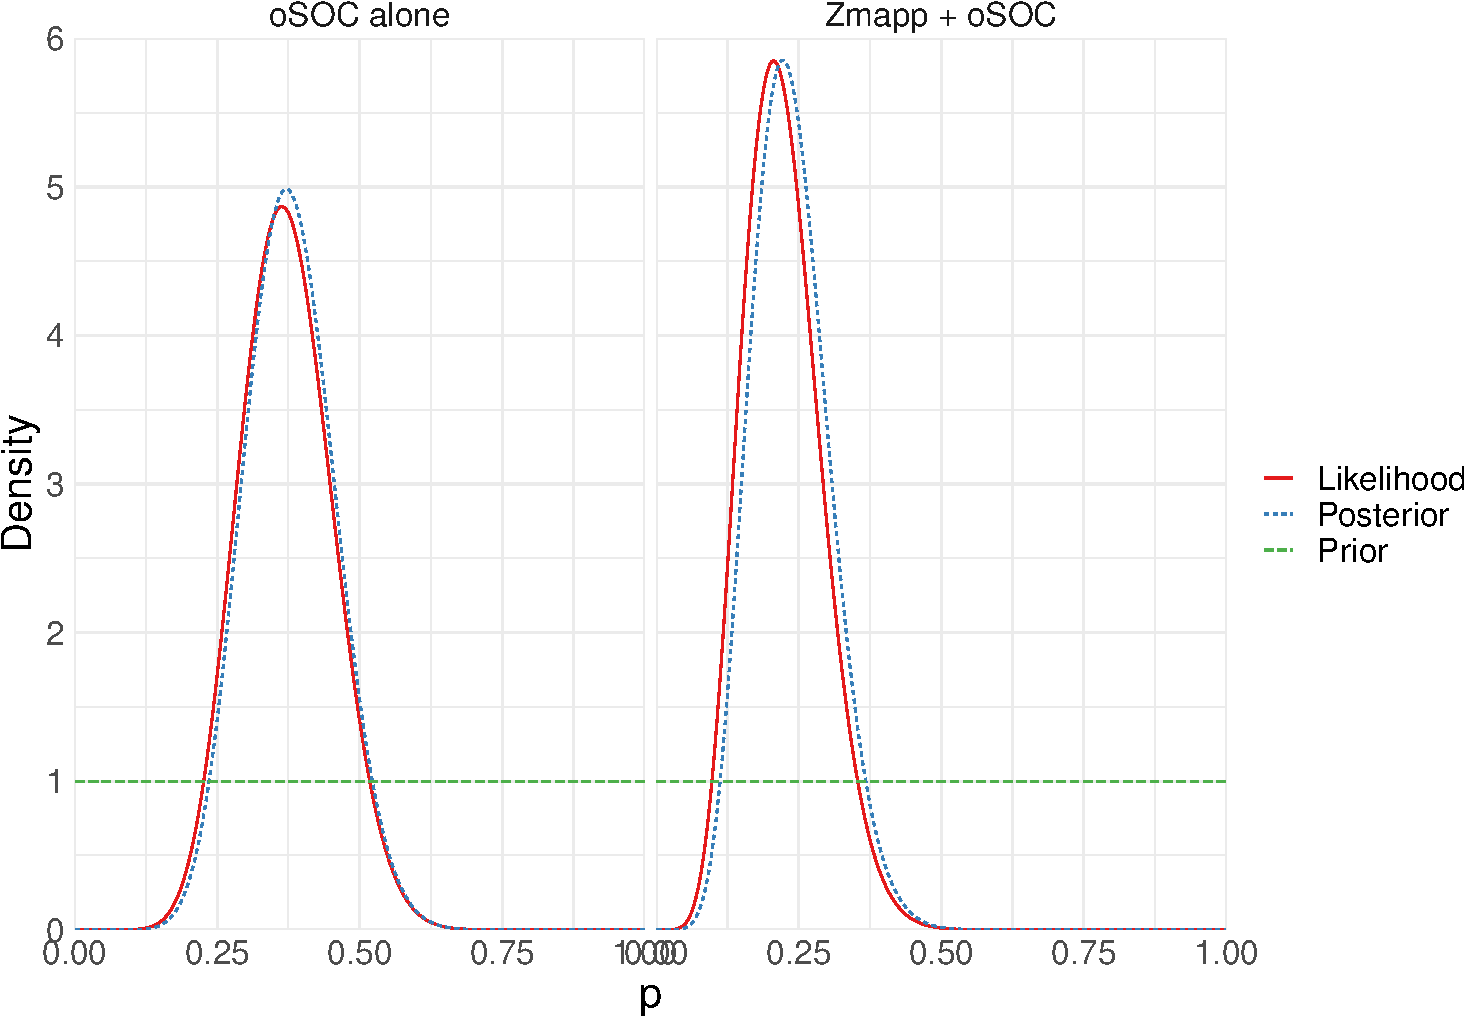
\includegraphics{sampling_probability_distributions_files/figure-beamer/prevail_posts-1.pdf}

\end{frame}

\begin{frame}{Posterior Mean and Likelihood-Prior Interaction}
\protect\hypertarget{posterior-mean-and-likelihood-prior-interaction}{}

\begin{itemize}
\tightlist
\item
  Recall the mean of a Beta\((a,b)\) is \(a/(a+b)\).
\item
  The posterior mean of a Beta\((y+a,N-y+b)\) is therefore
  \vspace{-0.1in} \begin{align*}
  \E(p|y) &= \frac{y+a}{N+a+b}\\
  &= \frac{y}{N+a+b} + \frac{a}{N+a+b}\\
  &= \frac{y}{N}\times \frac{N}{N+a+b} + \frac{a}{a+b}\times \frac{a+b}{N+a+b}\\
  &= \mr{MLE} \times \mr{W} + \mr{Prior Mean} \times (\mr{1-W}),\vspace{-0.1in}
  \end{align*} where the \emph{weight} W is
  \(\mr{W} = \frac{N}{N+a+b}.\)
\item
  As \(N\) increases, the weight tends to 1, so that the posterior mean
  gets closer to the MLE.
\item
  Notice that the uniform prior \(a=b=1\) gives a posterior mean of
  \(\E(p|y) = \frac{y+1}{N+2}.\)
\end{itemize}

\end{frame}

\begin{frame}{Choosing Prior Hyperparameters}
\protect\hypertarget{choosing-prior-hyperparameters}{}

\textbf{How to specify hyperparameters \(a\) and \(b\)?}\vspace{-0.1in}

\begin{itemize}
\tightlist
\item
  \emph{Suggestion \#1:} Use information about prior mean prior ``sample
  size.''

  \begin{itemize}
  \tightlist
  \item
    Prior mean: m\_\{prior\} = a/(a+b)\$.
  \item
    Recall, \(\E(p|y)=\frac{y+a}{N+a+b}\), so the denominator is like
    the posterior sample size, \(\implies N_{prior} = a+b.\).
  \item
    Solve for \(a\) and \(b\) via \vspace{-0.1in} \begin{align*}
      a &= N_{prior} \times m_{prior},\\
      b &= N_{prior} \times (1 - m_{prior}).
    \end{align*}
  \item
    \emph{Intuition}: view \(a\) and \(b\) as pseudo-observations of
    successes and failures.
  \end{itemize}
\item
  \emph{Suggestion \#2:} Choose \(a\) and \(b\) by specifying
  \emph{two quantiles} for \(p\) associated with prior probabilities.

  \begin{itemize}
  \tightlist
  \item
    e.g., \(\Pr(p<0.2) = 0.1 and \Pr(p > 0.6) = 0.1\).
  \item
    Can find values of \(a\) and \(b\) numerically.
  \item
    In more complicated models, simulate.
  \end{itemize}
\end{itemize}

\end{frame}

\begin{frame}{How to Specify Priors in General?}
\protect\hypertarget{how-to-specify-priors-in-general}{}

\textbf{Theme:} What aspects of my model do I know something about? How
do I encode that knowledge?\vspace{-0.1in}

\begin{itemize}
\tightlist
\item
  \textbf{Containment:} Does my prior predictive distribution produce
  realistic datasets?
\item
  \textbf{Caveat:} People who don't interrogate and justify their priors
  deserve what's coming to them.

  \begin{itemize}
  \tightlist
  \item
    Table of priors with references.
  \item
    Prior predictive checks.
  \item
    Sensitivity analyses.
  \end{itemize}
\end{itemize}

\end{frame}

\begin{frame}{Issues with Uniformity}
\protect\hypertarget{issues-with-uniformity}{}

We might think that if we have little prior opinion about a parameter
then we can simply assign a \textcolor{red}{uniform prior}, i.e.~a prior
\(p(\theta) \propto \mr{constant}.\)

There are two problems with this strategy:

\begin{itemize}
\tightlist
\item
  We can't be uniform on all scales since, if \(\phi = g(\theta)\):
  \[\underbrace{p_\phi( \phi )}_{\text{Prior for }\phi}  = \underbrace{p_\theta( g^{-1}(\phi) )}_{\text{Prior for } \theta} \times  \underbrace{\left|\frac{d \theta}{d \phi} \right|}_{\text{Jacobian}}\]
  and so if \(g(\cdot)\) is a nonlinear function, the Jacobian will be a
  function of \(\phi\) and hence not uniform (more on this in a bit).
\item
  If the parameter is not on a finite range, an
  \textcolor{red}{improper} distribution will result (that is, the form
  will not integrate to 1). This can lead to all kinds of paradoxes (see
  e.g., Dawid, 1973).
\item
  And importantly, improper priors are non-generative \(\implies\)
  cannot interrogate their predictive distribution.
\end{itemize}

\end{frame}

\begin{frame}{Are Priors Really Uniform?}
\protect\hypertarget{are-priors-really-uniform}{}

\begin{itemize}
\tightlist
\item
  In the binomial example, \(p\sim Unif(0,1)\) seems a natural choice.
\item
  But suppose we are going to model on the logistic scale so that
  \[\phi = \log\left( \frac{\theta}{1-\theta} \right)\] is a quantity of
  interest. -A uniform prior on \(\theta\) produces the very non-uniform
  distribution on \(\phi\). -Not being uniform on all scales is not a
  problem, and is correct probabilistically, but one should be aware of
  this characteristic.
\end{itemize}

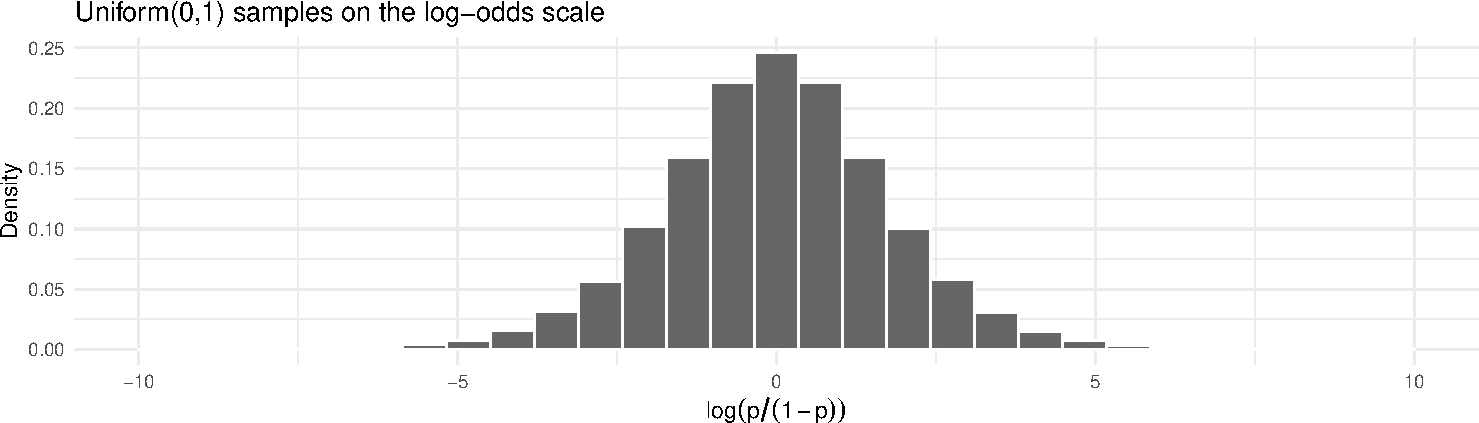
\includegraphics{sampling_probability_distributions_files/figure-beamer/logit_hist-1.pdf}

\end{frame}

\begin{frame}{Are Priors Really Uniform?}
\protect\hypertarget{are-priors-really-uniform-1}{}

\begin{itemize}
\tightlist
\item
  In the binomial example, \(p\sim Unif(0,1)\) seems a natural choice.
\item
  But suppose we are going to model on the logistic scale so that
  \[\phi = \log\left( \frac{\theta}{1-\theta} \right)\] is a quantity of
  interest. -A uniform prior on \(\theta\) produces the very non-uniform
  distribution on \(\phi\). -Not being uniform on all scales is not a
  problem, and is correct probabilistically, but one should be aware of
  this characteristic.
\end{itemize}

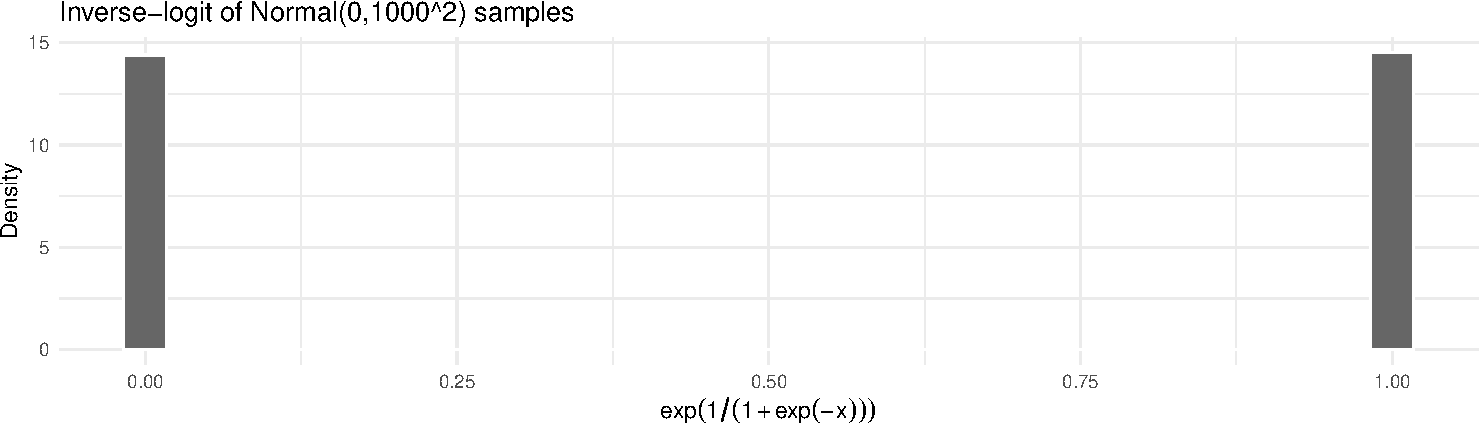
\includegraphics{sampling_probability_distributions_files/figure-beamer/expit_hist-1.pdf}

\end{frame}

\begin{frame}{Non-Conjugate Priors}
\protect\hypertarget{non-conjugate-priors}{}

Suppose we want to model mortality on the log-odds scale,
\(\theta = \log(p/(1-p))\).

Bayesian inference \emph{always} starts with a model for the
\textbf{joint distribution} of \(\theta\) and \(y\). \vspace{-0.1in}

\begin{itemize}
\tightlist
\item
  The parameter in our model is \(\theta\).
\item
  Lose conjugacy, no closed form for the posterior, now we rely on MCMC.
\item
  Our MCMC targets the posterior
  \(\pi(\theta|y)\propto \pi(\theta,y)=L(y|\theta)\pi(\theta).\)
\item
  If our prior is on the log-odds of death, we have no problems. It does
  not matter that \(L(y|\theta) = Binomial(N, 1/(1+exp(-\theta)))\).
\item
  If our prior is on the probability of death but our model is defined
  in terms of the log-odds, we must include a Jacobian adjustment.
\end{itemize}

\textbf{Critical:} We must never lose sight of how our model is defined.

For more on this, see case studies
\href{http://rstudio-pubs-static.s3.amazonaws.com/486816_440106f76c944734a7d4c84761e37388.html}{here}
and
\href{https://mc-stan.org/users/documentation/case-studies/mle-params.html}{here
study}.

\end{frame}

\begin{frame}{Why Non-Conjugate Priors?}
\protect\hypertarget{why-non-conjugate-priors}{}

\begin{itemize}
\tightlist
\item
  Information encoded naturally on other scales.
\item
  More flexible/natural representation using other types of
  distributions.
\item
  Hierachical information.
\item
  Compuational considerations.
\item
  Induce particular features in the posterior, e.g., sparsity.
\end{itemize}

\end{frame}

\begin{frame}{Next week}
\protect\hypertarget{next-week}{}

Linear regression. Watch lecture 3 (SmaRt).

We'll talk about:

\begin{itemize}
\tightlist
\item
  Bayesian linear regression.
\item
  Weekly informative priors.
\end{itemize}

\end{frame}

\begin{frame}{References}
\protect\hypertarget{references}{}

P.A. Dawid, M. Stone, and J.V. Zidek. ``Marginalization paradoxes in
Bayesian and structural inference.'' \emph{Journal of the Royal
Statistical Society: Series B (Methodological)} 35.2 (1973): 189-213.

A. Gelman, D.A. Simpson, and M. Betancourt. ``The prior can often only
be understood in the context of the likelihood.'' \emph{Entropy} 19.10
(2017): 555.

The PREVAIL II Writing Group and Multi-National PREVAIL II Study Team.
``A randomized, controlled trial of ZMapp for Ebola virus infection.''
\emph{The New England Journal of Medicine} 375.15 (2016): 1448.

M.A.~Proschan, L.E. Dodd, and D. Price. ``Statistical considerations for
a trial of Ebola virus disease therapeutics.'' \emph{Clinical Trials}
13.1 (2016): 39-48.

\end{frame}

\begin{frame}{}
\protect\hypertarget{section}{}

\end{frame}

\end{document}